\chapter{Spin, Measurement, and the Two-Dimensional State Space}

This lecture is presented as a review, but it is really a reorganization of the subject around its central difficulty. Leonard Susskind renames the qubit a spin, cleans up the distinction between ordinary three-vectors and abstract state-vectors, and then deliberately interrupts the march toward operators in order to talk about measurement and logic first. That order matters. The strange logic of quantum measurements is not an afterthought; it is the reason vector spaces enter at all. These notes follow that unfolding closely, with the surviving blackboard record kept visible where it clarifies the sequence of the argument. The lecture record itself is due to Leonard Susskind, with curation by LazyingArt LLC and Video2Book.

\section{From Qubit To Spin}

We begin with a change of language. The simple one-qubit system of the previous lecture will now be called a spin. Susskind also sharpens a distinction that we will need constantly from this point onward.

\begin{definition}
A \emph{three-vector} is a vector in ordinary real three-dimensional space. When we speak simply of a \emph{vector}, unless stated otherwise, we mean an element of an abstract vector space.
\end{definition}

This is not cosmetic terminology. The spin does seem to possess some kind of orientation in space, but the object that will ultimately describe its state is not itself an ordinary arrow in space. The lecture is constantly moving between these two meanings of the word \emph{vector}, and it is important not to let them blur together.

That clarification leads directly to the next point: the role of measurement. In classical physics one may idealize measurements as arbitrarily gentle. One can, in principle, find out what one wants to know about a system while disturbing it by an arbitrarily small amount. Quantum mechanics is not like that. Measurements inevitably disturb something. They do not necessarily destroy every fact about the system, but they do prevent us from pretending that a system and the apparatus measuring it can be discussed in complete isolation from one another.

That is why Susskind pauses here. Before returning to vector spaces and operators, he wants to talk first about the logic of the subject. The logic is different because the measurements are different.

\section{The Spin And The Apparatus}

Let us go back to the simplest operational picture. The spin is drawn as a little arrow, not because we have already proved that it is a classical arrow, but because anything we can draw on a blackboard will be classical-looking.

\begin{figure}
\centering

\includegraphics[width=0.58\textwidth]{lecture_02_figure_02.png}
\caption{Spin introduced as a single upward arrow.}
\end{figure}

We may echo the board's notation by writing
\[
\uparrow
\]
but the picture should be read cautiously. It is only a provisional visualization.

The apparatus is imagined as a device with a window that displays a number and with an orientation that tells us which way it is pointing. The crucial empirical fact is very simple: no matter how the apparatus is oriented, and no matter what has happened to the spin beforehand, the apparatus returns only two possible outcomes,
\begin{equation}
\sigma_{\hat m}=\pm 1,
\end{equation}
where \(\hat m\) denotes the orientation of the apparatus. When the apparatus points upward we say that it measures the \(z\)-component of spin, and when it points to the right we say that it measures the \(x\)-component. The lecture's convention is
\[
z \text{ up}, \qquad x \text{ to the right}, \qquad y \text{ out of the blackboard.}
\]

At this stage the word ``component'' is only a label. Susskind is explicit about this. We are not yet entitled to think of \(\sigma_z,\sigma_x,\sigma_y\) as classical components of an ordinary three-vector. All we know is that the apparatus, when pointed in any direction, answers with \(+1\) or \(-1\).

A measurement also serves as a preparation. If we point the apparatus upward and obtain \(+1\), then we say that the spin has been prepared ``up'' along the \(z\)-axis.

\subsection{Question \& Answer}

\paragraph{If measurements disturb systems, why do repeated measurements of the same component still reproduce the same result?}

Because quantum disturbance is not the statement that every measurement randomizes everything. Susskind's answer is: a measurement affects some things, but not that same thing. If we measure \(\sigma_z\) and obtain \(+1\), then measure \(\sigma_z\) again, with the same apparatus orientation and no intervention in between, we get \(+1\) again, and again. In that sense quantum mechanics still permits reproducible experiments.

This is not a minor remark. Without such reproducibility there would be no stable notion of preparation. A measurement both reveals and prepares: after the first \(z\)-measurement, the spin is definite with respect to the very same question.

\section{Direction Without Classical Components}

Now we test whether this object really has some notion of directionality. If we measure the spin with the apparatus pointing up and obtain \(+1\), then turn the apparatus completely over and measure again, we obtain \(-1\). That is not how a thermometer behaves. Turning a thermometer upside down does not make it measure minus the temperature. So already the spin is telling us that orientation matters.

The same is true when the apparatus is rotated sideways. We are then asking for what the lecture calls the \(x\)-component of the spin. The board stabilizes the notation as follows.

\begin{figure}
\centering

\includegraphics[width=0.72\textwidth]{lecture_02_figure_03.png}
\caption{Outcome labels for \(\sigma_z\) and \(\sigma_x\).}
\end{figure}

The upper \(\sigma_z\)-line is slightly cropped in the surviving frame, but the lecture's meaning is clear from the transcript and neighboring board states. A clean reconstruction is

\begin{figure}
\centering
\begin{tikzpicture}
\draw[->] (0,0) -- (2.2,0) node[right] {$x$};
\node[anchor=west] at (3.0,0.45) {$\sigma_z=\pm1$};
\node[anchor=west] at (3.0,-0.45) {$\sigma_x=\pm1$};
\end{tikzpicture}
\caption{Cleaned reconstruction of the component labels and the \(x\)-direction cue.}
\end{figure}

So the spin certainly responds to the orientation of the apparatus. But that does \emph{not} mean it is an ordinary unit vector. If a classical vector of unit length were measured along arbitrary axes, its components would range continuously from \(-1\) to \(+1\). Here the apparatus stubbornly refuses to produce anything except the extreme values \(\pm1\). That is the first major tension of the lecture: the spin behaves enough like something directional to invite the picture of an arrow, but it does not behave like a classical vector when one measures its components.

\subsection{Question \& Answer}

\paragraph{Does the little arrow mean that there is genuine geometric direction, or is it only a provisional visualization?}

It is only a visualization, and Susskind says so repeatedly. The board picture is classical because the board itself is classical. One should not infer too much from the drawing. What the experiments do justify is weaker and more interesting: they show that the spin carries directional information in an operational sense. Rotate the apparatus and the statistics change; turn the apparatus over and the sign flips. That much is real. But the individual measurement outcomes are still only \(\pm1\), and there is no classical geometry yet hiding inside a single event.

\section{Average Values Recover Vector-Like Behavior}

The next step is the key one. Suppose the spin has been prepared so that
\[
\sigma_z=+1.
\]
Now rotate the apparatus and measure \(\sigma_x\). The result is no longer fixed. Half the time it comes out \(+1\), and half the time it comes out \(-1\). Therefore
\begin{equation}
\langle \sigma_x\rangle=0.
\end{equation}
The same is true if the apparatus is rotated into the \(y\)-direction:
\begin{equation}
\langle \sigma_y\rangle=0.
\end{equation}

Thus a spin prepared up along \(z\) has vanishing average \(x\)- and \(y\)-components, even though every single run still gives only \(\pm1\). If instead the spin is prepared so that \(\sigma_x=+1\), then subsequent \(y\)- or \(z\)-measurements are likewise split evenly between \(+1\) and \(-1\).

Only after these special cases are on the table does Susskind generalize. Prepare the spin along a unit direction \(\hat n\), then measure along another unit direction \(\hat m\). Every individual run still yields only \(\pm1\), but the average value is
\begin{equation}
\langle \sigma_{\hat m}\rangle=\hat n\cdot \hat m=\cos\theta_{nm}.
\end{equation}
On the board, the formula appears in the shorter lecture notation
\begin{equation}
\langle \sigma_m\rangle=n\cdot m.
\end{equation}

\begin{figure}
\centering

\includegraphics[width=0.72\textwidth]{lecture_02_figure_04.png}
\caption{Average spin component written as \(\langle \sigma_m\rangle=n\cdot m\).}
\end{figure}

The surviving frame is strong here. The first handwritten symbol could be misread in isolation, but the transcript clearly supports \(n\cdot m\), and that is the form we should preserve.

There is a small terminological bump in the lecture at this point. Susskind insists that the quantity in angle brackets is an ordinary average over many runs, even though physicists also often call it an expectation value. The mathematical content is the standard one: repeat the experiment many times and take the mean.

The formula becomes more concrete if we write the probabilities explicitly. Let
\[
p_+=P(\sigma_{\hat m}=+1),\qquad p_-=P(\sigma_{\hat m}=-1).
\]
Then
\begin{align}
p_+ + p_- &= 1,\\
p_+ - p_- &= \langle \sigma_{\hat m}\rangle = \hat n\cdot \hat m.
\end{align}
Solving these two equations gives
\begin{equation}
p_+=\frac{1+\hat n\cdot\hat m}{2},\qquad
p_-=\frac{1-\hat n\cdot\hat m}{2}.
\end{equation}
So the apparatus never learns how to output a projection directly. It remains a \(\pm1\) machine. The classical-looking projection emerges only after averaging.

There is an important limiting case that the lecture draws attention to. If \(\hat n=\hat m\), then \(\hat n\cdot\hat m=1\). Since the outcomes can only be \(\pm1\), an average of \(+1\) means every single run gave \(+1\). Likewise, if \(\hat n=-\hat m\), every run gives \(-1\). The average law therefore contains the reproducibility statements as special cases.

\section{Quantum Logic Through Propositions}

At this point the lecture makes its most deliberate pivot. Before more vector spaces and operators, we are asked to think about logic. Classical logic can be modeled in terms of sets: the states of a classical system form a set, and a proposition corresponds to the subset of states for which the proposition is true.

Thus classical negation, conjunction, and inclusive disjunction are represented by
\begin{equation}
\neg A=A^c,\qquad
A\land B=A\cap B,\qquad
A\lor B=A\cup B.
\end{equation}

\begin{figure}
\centering
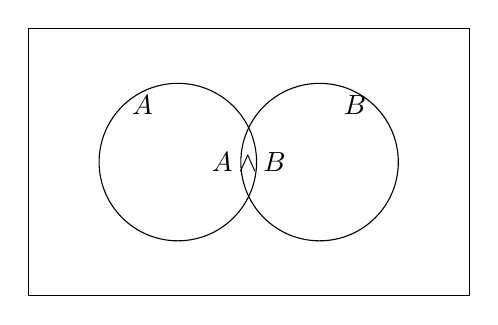
\begin{tikzpicture}
\draw (-2.8,-1.7) rectangle (2.8,1.7);
\draw (-0.9,0) circle (1.0);
\draw (0.9,0) circle (1.0);
\node at (-1.35,0.72) {$A$};
\node at (1.35,0.72) {$B$};
\node at (0,0) {$A\land B$};
\end{tikzpicture}
\caption{Classical propositions as subsets of a state-space.}
\end{figure}

Susskind pauses to emphasize that in logic the symbol \(\lor\) means the inclusive OR, not the everyday exclusive OR. If \(A\) is true, or \(B\) is true, or both are true, then \(A\lor B\) is true.

Now let us transport this language to the spin. Take the two propositions
\begin{equation}
A:\sigma_z=+1,\qquad B:\sigma_x=+1.
\end{equation}
Each can be checked individually without ambiguity. To check \(A\), we measure along the \(z\)-axis. To check \(B\), we measure along the \(x\)-axis. The trouble begins only when we ask how to verify the compound proposition \(A\lor B\).

\subsection{Question \& Answer}

\paragraph{How can \(A\lor B\) become order-dependent in quantum mechanics?}

To make the point as sharply as possible, Susskind imagines a ``ghost in the woodwork'' who has secretly prepared the spin with \(\sigma_z=+1\). We ourselves do not know this, but the hidden preparation lets us compare two verification procedures for the same compound statement.

If we test \(A\) first, then the very first measurement returns \(+1\). We are finished. Since \(A\) is true, the proposition \(A\lor B\) is certainly true.

Now reverse the order. Test \(B\) first. Since the spin was secretly prepared with \(\sigma_z=+1\), the first \(x\)-measurement gives \(+1\) or \(-1\) with equal probability:
\[
P(B\text{ true first})=\frac12,\qquad
P(B\text{ false first})=\frac12.
\]
But a measurement of \(B\) does not merely reveal an answer; it prepares the spin along the \(x\)-axis. So if the first result was not \(+1\), we must then check \(A\) on a spin that is now definite with respect to \(x\), not \(z\). The subsequent \(z\)-measurement is again random:
\[
P(A\text{ true after testing }B)=\frac12,\qquad
P(A\text{ false after testing }B)=\frac12.
\]
Therefore the probability that both tests fail is
\begin{equation}
P(\neg B\text{ and then }\neg A)=\frac12\cdot\frac12=\frac14.
\end{equation}

So in one order, \(A\lor B\) is certainly true; in the reversed order, it has a \(25\%\) chance to come out false. That is the phenomenon the lecture wants us to see. In classical logic, \(A\lor B\) is symmetric in \(A\) and \(B\). In quantum mechanics, any operational meaning given to the verification of \(A\lor B\) depends on the order in which the tests are carried out.

This is not merely the bland statement that ``measurements disturb systems.'' The sharper statement is that compound propositions inherit that disturbance and cease to have the classical symmetry one naively expects. Susskind allows the more technical summary that propositions correspond to projection operators, and projection operators need not commute:
\begin{equation}
P_A P_B \neq P_B P_A.
\end{equation}
That is not yet a full operator theory, but it is the right mathematical slogan for the logical obstruction.

\section{Why Vector Spaces Enter}

Only after the logical obstruction has been exposed does the lecture return to vector spaces. This timing is essential. Linear algebra is not being pasted on top of the physics as an abstract formal language; it is being introduced because the distorted quantum logic lives naturally inside the structure of a complex vector space.

The essential ingredients are the familiar ones. Vectors can be added. They can be multiplied by complex numbers. Every ket-vector has a corresponding bra-vector, and a bra may be paired with a ket to produce an inner product. If \(|A\rangle\) and \(|B\rangle\) are state-vectors, then
\begin{equation}
\langle A|B\rangle=\langle B|A\rangle^{*}.
\end{equation}
The square of the length of a vector is
\begin{equation}
\langle A|A\rangle,
\end{equation}
and this quantity is real and nonnegative. Two vectors are orthogonal when
\begin{equation}
\langle A|B\rangle=0.
\end{equation}

Dimension is then defined in the way Susskind likes to emphasize: it is the maximum number of mutually orthogonal vectors one can find in the space. In a two-dimensional complex vector space one can find two mutually orthogonal vectors, but no third one independent of them.

For the simple spin, the postulate is that the state-space is precisely such a space:
\begin{equation}
\mathcal H_{\text{spin}}\cong \mathbb C^2.
\end{equation}
That postulate summarizes a great deal. It says that although the apparatus may be pointed in continuously many directions, the abstract state-space of the single spin is nevertheless two-dimensional. The different prepared states are not separate dimensions; they are different vectors in the same two-dimensional complex space.

\section{Constructing The Spin State Space}

We now build the state-space explicitly, in the same heuristic order as the lecture itself. The style here is intentionally provisional. Susskind is not pretending to derive everything from a finished formalism; he is guessing, checking, and refining the vectors so that they reproduce the measurement facts.

\subsection{The \(z\)-basis}

We begin with the states prepared by an apparatus aligned with the \(z\)-axis. The lecture insists that the same state may be written in several different ``languages'': as a word, as a sign, as a little arrow, and as a \(\sigma\)-statement.

\begin{figure}
\centering

\includegraphics[width=0.72\textwidth]{lecture_02_figure_05.png}
\caption{Up/down notation translated into \(\sigma_z\)-language.}
\end{figure}

A clean reconstruction of the row-wise board dictionary is
\begin{align}
u \qquad &+ \qquad \uparrow \qquad \sigma_z=+1 \qquad |u\rangle,\\
d \qquad &- \qquad \downarrow \qquad \sigma_z=-1 \qquad |d\rangle.
\end{align}
The completion \(\sigma_z=+1\) in the first row is partly obscured in the surviving frame, but it is clearly supported by the spoken lecture and by the later board state.

These two states are not negatives of one another. They are orthogonal:
\begin{equation}
\langle u|d\rangle=0.
\end{equation}
The physical reason is the lecture's operational criterion: if two states can be distinguished unambiguously by an experiment, then they are orthogonal. A \(z\)-measurement distinguishes \(|u\rangle\) from \(|d\rangle\) with certainty.

Since the space is assumed to be two-dimensional, any state can be expanded in this basis:
\begin{equation}
|A\rangle=\alpha_u|u\rangle+\alpha_d|d\rangle,
\end{equation}
with \(\alpha_u,\alpha_d\in\mathbb C\).

The transcript is slightly garbled when Susskind states the probability rule, but the intended content is standard and clear:
\begin{equation}
P(u)=|\alpha_u|^2,\qquad P(d)=|\alpha_d|^2.
\end{equation}
Because probabilities must add to one,
\begin{equation}
|\alpha_u|^2+|\alpha_d|^2=1.
\end{equation}
This is exactly the normalization condition \(\langle A|A\rangle=1\), as one sees by using the orthonormality of \(|u\rangle\) and \(|d\rangle\):
\begin{align}
\langle A|A\rangle
&=
(\alpha_u^*\langle u|+\alpha_d^*\langle d|)
(\alpha_u|u\rangle+\alpha_d|d\rangle)\\
&=
|\alpha_u|^2\langle u|u\rangle
+\alpha_u^*\alpha_d\langle u|d\rangle
+\alpha_d^*\alpha_u\langle d|u\rangle
+|\alpha_d|^2\langle d|d\rangle\\
&=
|\alpha_u|^2+|\alpha_d|^2.
\end{align}
Thus physical states correspond to normalized vectors.

\subsection{Question \& Answer}

\paragraph{In what sense are \(|u\rangle\) and \(|d\rangle\) orthogonal if the pictures ``up'' and ``down'' lie on one line in ordinary space?}

Because orthogonality here is not ordinary perpendicularity in real space. The lecture eventually sharpens this point: in the space of states, orthogonality means physical distinguishability. \(|u\rangle\) and \(|d\rangle\) are orthogonal because a single well-designed experiment can tell them apart without ambiguity. By contrast, \(|u\rangle\) and \(|r\rangle\) are not orthogonal: a \(z\)-measurement on \(|r\rangle\) can still return ``up'' with probability \(1/2\). In that sense they overlap.

The safest rule is therefore this: do not confuse orthogonality in state-space with orthogonality of arrows in three-dimensional space.

\subsection{The \(x\)-basis: right and left}

Now rotate the apparatus into the \(x\)-direction. This gives two new states, right and left, corresponding to \(\sigma_x=+1\) and \(\sigma_x=-1\).

\begin{figure}
\centering

\includegraphics[width=0.74\textwidth]{lecture_02_figure_06.png}
\caption{The \(z\)-basis dictionary extended toward the \(x\)-basis states.}
\end{figure}

The board layout is important here: the \(z\)-basis rows remain at the top while a second, lower row begins for the left-right states. A clean reconstruction is

\begin{figure}
\centering
\begin{tikzpicture}
\node[anchor=west] at (0,1.1) {$u \qquad + \qquad \uparrow \qquad \sigma_z=+1$};
\node[anchor=west] at (0,0.3) {$d \qquad - \qquad \downarrow \qquad \sigma_z=-1$};
\draw[->] (1.2,-0.9) -- (2.5,-0.9);
\draw[->] (4.0,-0.9) -- (2.7,-0.9);
\node[anchor=west] at (4.5,-0.9) {$\sigma_x=\pm1$};
\end{tikzpicture}
\caption{Cleaned reconstruction of the board as the \(x\)-basis is introduced.}
\end{figure}

Let us denote the corresponding states by
\[
|r\rangle \leftrightarrow \sigma_x=+1,
\qquad
|l\rangle \leftrightarrow \sigma_x=-1.
\]

Now comes the lecture's characteristic move: we know \(|r\rangle\) must be some linear combination of \(|u\rangle\) and \(|d\rangle\), so let us write
\[
|r\rangle=\alpha_u|u\rangle+\alpha_d|d\rangle.
\]
What do we know about the coefficients? If the spin is prepared in the right state and we then measure up or down, each occurs with probability \(1/2\). Therefore
\[
|\alpha_u|^2=\frac12,\qquad |\alpha_d|^2=\frac12.
\]
The simplest guess is
\begin{equation}
|r\rangle=\frac{1}{\sqrt2}\bigl(|u\rangle+|d\rangle\bigr).
\end{equation}

What about \(|l\rangle\)? Right and left are unambiguously distinguishable by a single \(x\)-measurement, so they must be orthogonal. The natural candidate is
\begin{equation}
|l\rangle=\frac{1}{\sqrt2}\bigl(|u\rangle-|d\rangle\bigr).
\end{equation}
Indeed,
\begin{equation}
\langle l|r\rangle
=
\frac12(\langle u|-\langle d|)(|u\rangle+|d\rangle)
=
\frac12(1-1)=0.
\end{equation}

Thus the \(x\)-basis is
\begin{align}
|r\rangle &= \frac{1}{\sqrt2}\bigl(|u\rangle+|d\rangle\bigr),\\
|l\rangle &= \frac{1}{\sqrt2}\bigl(|u\rangle-|d\rangle\bigr).
\end{align}
Adding and subtracting these relations gives the inverse formulas
\begin{align}
|u\rangle &= \frac{1}{\sqrt2}\bigl(|r\rangle+|l\rangle\bigr),\\
|d\rangle &= \frac{1}{\sqrt2}\bigl(|r\rangle-|l\rangle\bigr).
\end{align}
This reciprocity is one of the points the lecture emphasizes: had we started our experiments with the apparatus aligned along \(x\), we might have taken \(|r\rangle\) and \(|l\rangle\) as basic and then discovered that \(|u\rangle\) and \(|d\rangle\) were their linear combinations.

\subsection{The \(y\)-basis: in and out}

Finally the apparatus is turned along the \(y\)-axis, giving the states ``in'' and ``out'' of the blackboard:
\[
|i\rangle \leftrightarrow \sigma_y=+1,
\qquad
|o\rangle \leftrightarrow \sigma_y=-1.
\]
Here the notation deserves one warning. The ket \(|i\rangle\) denotes the in-state, while the plain symbol \(i\) remains the imaginary unit. The lecture itself briefly stumbles over this collision of notation.

Again we proceed heuristically. Equal up/down probabilities require equal moduli of the coefficients, and orthogonality requires the pair to be mutually orthogonal. The lecture states the answer:
\begin{align}
|i\rangle &= \frac{1}{\sqrt2}\bigl(|u\rangle+i|d\rangle\bigr),\\
|o\rangle &= \frac{1}{\sqrt2}\bigl(|u\rangle-i|d\rangle\bigr).
\end{align}
The orthogonality check is straightforward. In the \((u,d)\)-basis,
\[
|i\rangle=\frac{1}{\sqrt2}\binom{1}{i},
\qquad
|o\rangle=\frac{1}{\sqrt2}\binom{1}{-i},
\]
so
\begin{equation}
\langle i|o\rangle
=
\frac12\left(1+(-i)(-i)\right)
=
\frac12(1-1)
=
0.
\end{equation}

The lecture then worries, a little theatrically, about whether these states are also symmetrically related to the \(x\)-basis. One can verify this neatly by rewriting \(|i\rangle\) in terms of \(|r\rangle\) and \(|l\rangle\):
\begin{align}
|i\rangle
&=
\frac{1}{\sqrt2}
\left(
\frac{|r\rangle+|l\rangle}{\sqrt2}
+
i\frac{|r\rangle-|l\rangle}{\sqrt2}
\right)\\
&=
\frac{1+i}{2}|r\rangle+\frac{1-i}{2}|l\rangle.
\end{align}
Now
\begin{equation}
\left|\frac{1+i}{2}\right|^2=\left|\frac{1-i}{2}\right|^2=\frac12,
\end{equation}
so a spin prepared in the in-state has probability \(1/2\) to be found right and probability \(1/2\) to be found left. The same holds for \(|o\rangle\). This is the symmetry the lecture was aiming at when it said that the three basis pairs are ``nicely symmetrically related.''

The standard column-vector representatives in the \((u,d)\)-basis are therefore
\begin{align}
|u\rangle &= \binom10,
&
|d\rangle &= \binom01,
\\
|r\rangle &= \frac{1}{\sqrt2}\binom11,
&
|l\rangle &= \frac{1}{\sqrt2}\binom1{-1},
\\
|i\rangle &= \frac{1}{\sqrt2}\binom1{i},
&
|o\rangle &= \frac{1}{\sqrt2}\binom1{-i}.
\end{align}

The lecture then asks whether there could be a fourth pair, as symmetrically related to the first three as they are to one another. The answer is no. That absence is deeply tied to the fact that ordinary space has three dimensions. The striking fact is that the continuously many spatial directions of a spin are being represented inside a two-dimensional complex state-space.

\subsection{Phase Indifference And Parameter Count}

How much information in the pair \((\alpha_u,\alpha_d)\) is physically meaningful? Two complex amplitudes contain four real parameters, but two of them are redundant.

First, normalization removes one parameter:
\begin{equation}
|\alpha_u|^2+|\alpha_d|^2=1.
\end{equation}
Second, the overall phase has no physical effect. If we multiply the whole state by a common phase factor,
\begin{equation}
|A\rangle \longmapsto e^{i\theta}|A\rangle,
\end{equation}
then all measurable probabilities remain unchanged. Thus the counting is
\begin{equation}
4\text{ real parameters}
-
1\text{ normalization}
-
1\text{ overall phase}
=
2\text{ real parameters}.
\end{equation}

This is the lecture's closing conceptual bridge. A direction in ordinary three-dimensional space is also specified by two real numbers, for example two angles. The agreement is not accidental. It is a first glimpse of the deep relation between a normalized two-component spin state and a direction in real space.

At the same time, Susskind is careful not to overclaim. We are not yet deriving that relation rigorously. We are finding vectors that fit the experiments, and discovering that they fit astonishingly well.

\section{Summary}

The lecture has unfolded in a very definite order. We began with operational facts: an oriented apparatus measures only \(+1\) or \(-1\), repeated measurements of the same component are reproducible, and rotating the apparatus changes the statistics in a way that shows genuine directional structure. We then saw the central tension: the spin behaves directionally, but not by having classical components event by event. Classical vector behavior reappears only in averages, through
\[
\langle \sigma_{\hat m}\rangle=\hat n\cdot\hat m.
\]

From there the lecture pivoted to logic. The compound proposition \(A\lor B\), with \(A:\sigma_z=+1\) and \(B:\sigma_x=+1\), does not behave classically under verification. Its operational meaning depends on the order of testing. That logical distortion is what leads us to vector spaces.

Finally, the lecture built the two-dimensional complex state-space of a single spin. The \(z\)-basis states \(|u\rangle,|d\rangle\), the \(x\)-basis states \(|r\rangle,|l\rangle\), and the \(y\)-basis states \(|i\rangle,|o\rangle\) were constructed as a coherent family of normalized vectors reproducing the measurement facts. The picture is already powerful, but it is still heuristic. The lecture ends by saying so plainly: we have been guessing, checking, and testing. The next step is to make rigorous the relation between these state-vectors and the observables \(\sigma_x,\sigma_y,\sigma_z\).